\chapter{Simulation Results}
\textbf{Content}: Comparison of flooding to petal routing on the basis of delivery ratio, end-to-end delay, overhead, average number of hops. 
\textbf{Intent}:  Present data and analysis for the performance of petal routing.

We have used Qrsim quadrotor simulator \cite{denardi2013rn} - briefly explained in section \ref{qrsim_intro} - for evaluating our protocol. The volume of the simulated flying zone is 120 units $ \times \text{120 units} \times \text{120 units, out of which we have used 80 units} \times \text{80 units}\times $ 50 units where drones can be placed. We also have a scaling factor which scales the simulation units i.e. a scaling factor of 20 will make 1 unit in simulation to 20 meters. The simulation state changes at a time quantum of 0.2 seconds.

Initially, the drones start in a mesh formation arranged in a 2D grid as shown in \fref{fig:mesh_formation} and gradually they wrap around the plume - which, in our case, for simplicity, has been assumed to be spherical \fref{fig:final_state}. Besides these two formations, we have also evaluated our results for a random distribution of drones in the simulation space \fref{fig:random_formation}.

\begin{figure}[hbtp]
\centering
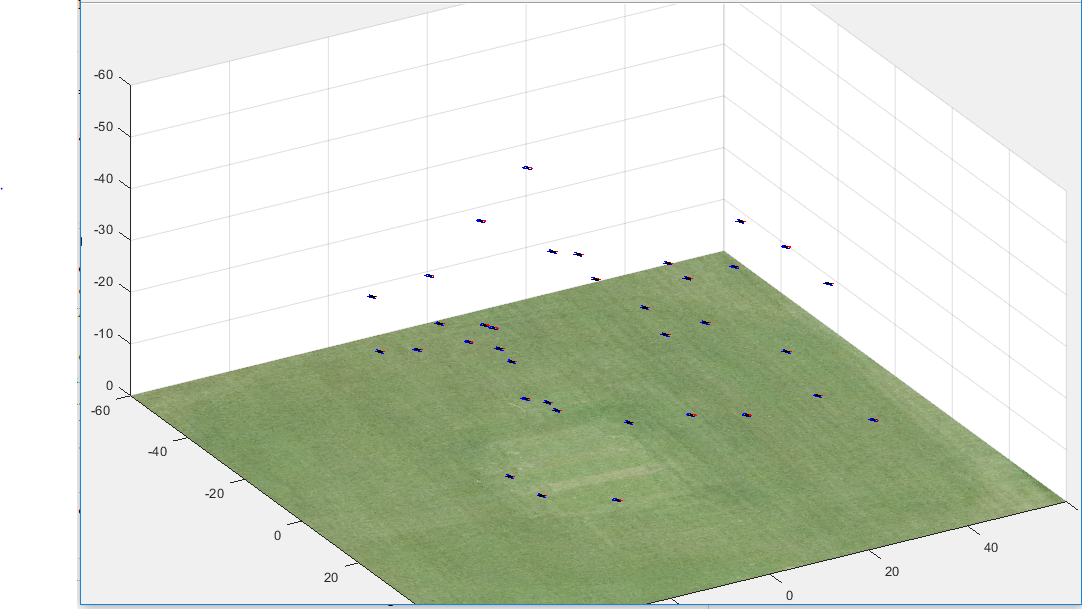
\includegraphics[width=0.8\textwidth]{ncsuthesis-0.6/Chapter-5/figs/random_drone_locations}
\caption{Random distribution of UAVs in the simulation space}
\label{fig:random_formation}
\end{figure}

The messages sent among the drones are assumed to be small and we have not considered transmission errors and congestion separately, rather they are assumed to be represented by the free space path loss model explained in section \ref{free_space_path_loss}. We have picked 200 furthest pairs of drones for our result evaluation. 

In the following sections we compare the performance of the two schemes of our routing protocol to flooding algorithm. The x axis for 
\section{Delivery ratio}
\section{Average number of hops}
\section{Average end to end delay}
\section{Average number of transmissions}
\section{Scalability}
\section{Effect of node density}

\textbf{Node density:} Assuming that a perfectly omnidirectional antenna can deliver packets directly and reliably to a receiver at a distance of $ r meter$  in space, then the volume covered by the transmitter would be $ v = \dfrac{4}{3} \cdot \pi \cdot r^3 $. Considering the volume of the flying space is V, and the number of drones in the space is DC, we classify the node density of the simulation as sparse, ideal and high according to the following relation.

\begin{eqnarray} \label{node_density}
\begin{aligned}
& \text{Sparse node density:} & \dfrac{V}{v} << DC \\
& \text{Ideal node density:} & \dfrac{V}{v} \approx DC \\
& \text{High node density:} & \dfrac{V}{v} >> DC
\end{aligned}
\end{eqnarray}

For example, with scaling factor = 20, Number of Drones = 36, and flying space volume = $ 80 \times 80 \times 40 unit^3  \text{and } r = 250 m $,
\begin{eqnarray*}
& \text{we have,} & V = 80 \times 80 \times 40 \times 20 \times 20 \times 20 = 2048000000 unit^3 \\
& {and} & v = \dfrac{4 \times 3.14 \times 250 ^ 3}{3} = 65416667 unit ^ 3 \\
& \Rightarrow & \dfrac{V}{v} \approx 31
\end{eqnarray*}